%TC:envir minttcb [ignore] xall

\chapter{Introduction}\label{chp:intro}

Electrically powered vertical takeoff and landing (eVTOL) aircraft could provide a new mode of air transportation of people and cargo that is low-cost, on-demand, and able to reach more areas than is possible with current technology. Winged eVTOLs, or simply eVTOLs, are a class of aerial vehicles that can travel using aerodynamic lift yet take off and land vertically. This means eVTOLs don't require runways or other large infrastructure to operate; they can take off and land virtually anywhere, even in compact or congested spaces. They are much more energy-efficient than most vertically flying aircraft, like helicopters and multirotors, because of the aerodynamic lift produced by their wings during horizontal flight. This gives them the ability to travel longer distances and carry heavier payloads. With these advantages, there is great interest in eVTOLs as a cost-effective technology for rapid, point-to-point air transportation of people and cargo.

\begin{figure}[h]
    \centering
    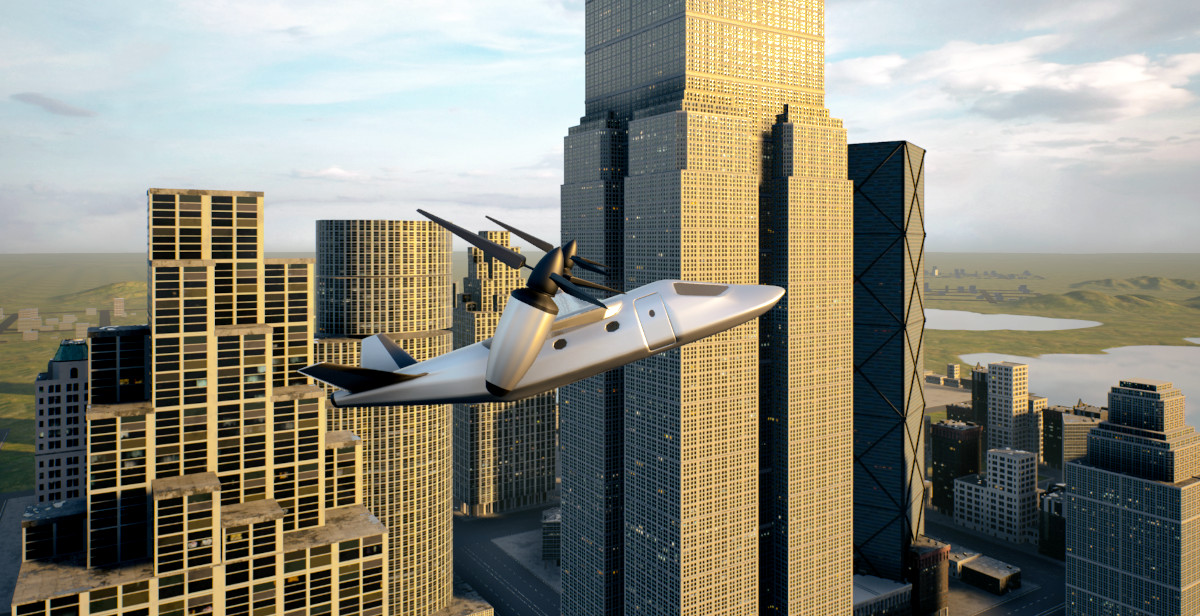
\includegraphics[width=\textwidth]{figures/vtol_airsim_cityblocks_crop3}
    \caption[Tiltrotor vehicle in CityBlocks environment]{
        \textit{VTOL-AirSim}: our tool for simulating eVTOL aircraft in realistic environments.}%
    \label{fig:vtol_airsim_cityblocks}
\end{figure}

Advancements in computing power, electronics, digital sensors, and software have enabled great progress towards increasingly automated flight of these aircraft, which is further made possible by their fully electric propulsion. With autonomous flight capabilities, eVTOLs will have greater safety, efficiency, and ease of operation. Key to the research and development of autonomous vehicles is the ability to simulate their control and navigation software; however, because they have only recently become a possibility, the field of eVTOL research is less mature, and simulators with support for eVTOLs are scarce.

Many modern unmanned aerial vehicles (UAVs) that can fly autonomously rely on camera sensors. This is because visual data contains a large amount of information about the environment that can be used to detect and avoid obstacles, navigate through cluttered spaces, and identify and track targets. It is therefore important to simulate vision-based navigation for eVTOLs. Simulating visual data from a camera sensor, however, requires high-fidelity graphics to accurately test the performance of the vision-based navigation software. There are few publicly available simulators which utilize high-quality graphics engines, and this further complicates finding a viable simulator for eVTOLs.


This thesis explains our contribution of creating a capable, high-graphics simulation of winged eVTOL aircraft that others can use. In addition, we show a system that we developed for others to easily create their own unique simulations of eVTOLs. The simulation we developed is an extension of Microsoft AirSim, a popular open-source tool used by many researchers for simulating multirotor aircraft.

\section{Review of Available Simulation Tools}
To the best of our knowledge, there are currently no publicly available simulators for research that provide the ability to simulate eVTOL aircraft with high-quality graphics. Therefore, it was necessary for us to choose from the simulation tools that are available and design a way to modify, extend, or otherwise work around these tools to produce something that they currently do not offer.

There are two well-known products in the world of flight simulation that are renowned for their high-fidelity graphics, massive amount of features, and accurate modeling of the physics of flight: \textit{Microsoft Flight Simulator}~\cite{Microsoft2020}, and \textit{X-Plane 11} from Laminar Research~\cite{X-plane112020}. While different, these two products fit into similar categories as simulation tools. A brief comparison of the two are given in~\cite{Gimenes2008}. They offer creating customized aircraft, but with different implementations. The flight model in Flight Simulator uses a set of tables which are computed by supplied parameters. X-Plane 11 computes flight dynamics directly from the visual model, and it allows for the use of one's own flight model, in which case the aircraft becomes just a visual representation of the externally simulated dynamics. The latter is advantageous in the case of simulating an eVTOL aircraft, in which the dynamic model can greatly differ from that of standard fixed-wing, helicopter, or multirotor aircraft. However, neither software allows for winged eVTOL designs, such as animating tiltable rotors. This is undesirable --- not only for the purpose of presenting simulations to others, but also for the engineering analysis and insight that is lost when using a visualization that misrepresents core components. In addition, both simulators are closed-source, proprietary software products that are heavily geared toward simulating the piloting of aircraft rather than tools for researching autonomous navigation software for UAVs. They don't provide easy-to-use, flexible programming interfaces to accommodate typical software written by researchers. Despite this, some researchers have found them useful as UAV simulators, due to their high fidelity graphics and flight dynamics, such as the use of Microsoft Flight Simulator in~\cite{Marcu2011},~\cite{Louali2011} and the use of X-Plane in~\cite{Garcia2010},~\cite{Cho2021}. Note that these studies only simulated standard fixed-wing or helicopter aircraft.

A simulator that has arguably become the standard simulator for robotics research is the free and open-source Gazebo project~\cite{Koenig2004}. It is widely used in both robotics and UAV research and thus has a large community. It is highly customizable, even to allow for simulating eVTOLs, as in~\cite{Carlson2021}. However, this comes at the cost of requiring a great deal of manual setup on the part of the researcher, as Gazebo is a rather generic robotics simulator and does not offer built-in features such as eVTOL aircraft. In addition, the graphics quality of simulations made in Gazebo are, by today's standards, of moderate or low fidelity. This makes it less useful for accurately simulating vision-based navigation and control.

Another simulator from Microsoft, \textit{AirSim}~\cite{Shah2018}, is becoming increasingly popular among multirotor UAV researchers. It is free, open-source, and is built on \textit{Unreal Engine}~\cite{Games2020}, a professional game engine from Epic Games that is known for its very high-quality graphics. It has many built-in features, such as support for the PX4 Autopilot~\cite{Meier2015} and ROS~\cite{OpenRobotics2013}, and it provides simple interfaces in Python and \CCd. It also offers a number of prebuilt environments of high-quality graphics that can be downloaded and ran on anyone's machine in a number of minutes. AirSim has been used for simulating vision-based navigation in~\cite{Ruf2018},~\cite{Bondi2018},~\cite{Meier2015}. A core problem with AirSim is that it's completely structured around three separate simulation modes: Multirotor, Car, or Computer Vision (i.e., a camera with no dynamics or vehicle). This means that eVTOL aircraft, or even fixed-wing vehicles, can not be simulated in AirSim. Moreover, while AirSim is open-source and does contain documentation on how to customize it, doing so requires installing and using Unreal Engine, which has high computer hardware requirements and a steep learning curve.

And finally, there is the \textit{ROSflight Holodeck} simulation system. This is a tool developed by the MAGICC Lab that combines two other projects, the ROSflight autopilot created by former students of the MAGICC Lab, and the Holodeck simulator, created by the BYU Perception, Control, and Cognition Lab, into a full software-in-the-loop simulation with a high-quality graphics environment. Like AirSim, Holodeck uses Unreal Engine for its graphics, and thus can be a great tool for computer vision applications. In contrast to AirSim, the project's sole developers are a few graduate students, and it currently lacks many important features, such as support for multiple vehicles.

For our solution, we chose to develop an extension to Microsoft AirSim that adds the capability of simulating eVTOL aircraft, which we gave the name of \textit{VTOL-AirSim}.

\section{Contributions}

This thesis makes contributions in the following areas:

\begin{itemize}
    \item An extension to AirSim for simulating eVTOL aircraft control and dynamics, named VTOL-AirSim. It includes high-quality graphics for realistic simulated camera images. We also created visual components for the simulation: a fully animated tiltrotor aircraft mesh, and a detailed city environment to fly it in. An introduction to AirSim and tutorials for VTOL-AirSim, which includes scripts we created for interfacing VTOL-AirSim with a trajectory generator, a geometric controller and an eVTOL control allocation module from the MAGICC Lab's VTOLsim project~\cite{Willis2021},~\cite{Willis2022}, are given in Chapter~\ref{chp:userguide}. A tutorial for interfacing the PX4 Autopilot with VTOL-AirSim is also given in that chapter.
    \item A guide on all the tools that are needed to extend VTOL-AirSim is given in Chapter~\ref{chp:extending}. We show how to build Unreal Engine from source and install it on Linux, after which we provide a short user guide.
    \item Tutorials for creating custom aircraft and custom environments for use in VTOL-AirSim are given in Chapters~\ref{chp:custom_aircraft} and~\ref{chp:custom_envs}, respectively. We provide full examples of how to obtain prebuilt content from online and then integrate the content using the Unreal Editor to create a customized VTOL-AirSim simulation.
\end{itemize}